\documentclass[11pt]{article}
\usepackage{colacl}
\usepackage{graphicx}
\sloppy


\title{COMP30027 Report}
\author
{Anonymous}



\begin{document}
\maketitle


%\begin{abstract}
%Don't include an abstract.
%\end{abstract}

\section{Introduction}


\section{Methodology}

\subsection{Understanding the Data}
\subsubsection{Class Distribution} 
By counting the frequency of each class and understanding the distribution of the classes in the training data, we can gain valuable insights when designing and evaluating models.

\subsection{Data Preprocessing}

\subsubsection{Normalisation}
For most of the numeric values in the dataset, the important information is how it compares to other values, rather than the actual value itself. These values should be normalised. Since some models prefer 0 mean data, such as logistic regression and support vector machines, standardisation will be the normalisation method of choice. However, attributes like \texttt{title\_year} or \texttt{average\_degree\_centrality} are more valuable as the value itself, and so these will not be standardised.

\subsubsection{Removing Highly Correlated Attributes}
There are a few reasons to remove all but one attribute from a set of highly correlated attributes. Not only does removing the attributes decrease dimensionality and makes the models faster, but having multicollinearity among independent variables can result in less reliable statistical inferences. By removing them, we should be able to increase the models' ability to generalise and not overfit to the training data.


\subsubsection{Dropping Unuseful Values}
Considering that the data is likely to be biased towards certain regions of the world, there will likely be certain attributes the exhibit an overwhelming majority of one variation, with many other unique but less prevalent values. These attributes would not be very useful to the data, and the best way to approach them is dropping them from the dataset. This also has the additional advantage of decreasing the dimensionality of the data, and hence increasing the speed of the models.

\subsubsection{One Hot Encoding}

\subsection{Baseline Models}
To provide a baseline for benchmarking, we can develop a few simple models. The simplest that can be developed is just a model that guesses the most common class. Following this, a One Rule model could be developed on the categorical attributes, such as film categories.

\subsection{Model Design}
\subsubsection{Models}

Three models were picked, these were:

\begin{itemize}
    \item Support Vector Machine
    \item Logistic Regression
    \item Random Forest
\end{itemize}

For each of the models, the below steps were followed to find the best model:

\begin{enumerate}
    \item The training data was split into a training set and validation set.
    \item For each hyperparameter model, a few reasonable options were selected.
    \item Iterating over all combinations of hyperparameters, the combination that resulted in the highest accuracy over the training set was picked.
    \item The model is evaluated over the validation set.
    \item Using sequential forward selection and the best hyperparameters for the model, the best combination of features is selected for the training of the model. 
    \item Using the best hyperparamters and best features, the model is evaluated against 

\end{enumerate}



\section{Results}

\subsection{Class Distribution}
Figure~\ref{fig:class-dist} shows the distribution of the classes in the training dataset. It's clear that a rating of 2 is by far the most common, followed by 3. However, it's only a 61.2\% majority, which means a model that always guesses 2 won't have the best accuracy.

\begin{figure}[!ht]
	\centering
	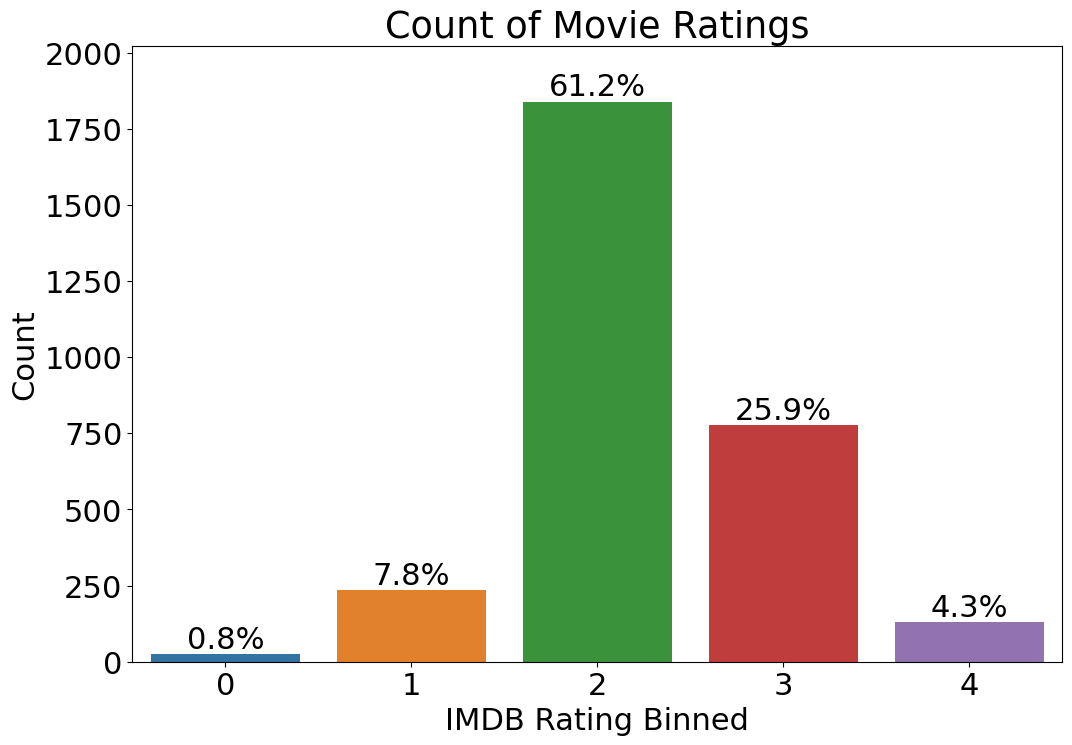
\includegraphics[width = 0.48\textwidth]{res/class-dist.png}
	\caption{Count plot showing the distribution of classes in the training data}
	\label{fig:class-dist}
\end{figure}

\subsubsection{Category One Rule}



\subsection{Preprocessing}

\subsubsection{Unhelpful Features}
Since most films are in english and there are many other unique values with very low frequency, the language feature is not very useful and should be dropped. A similar occurence also exists with the country feature, where the USA is an overwhelming majority. 

\ 

\noindent
Similarly, a large majority of movies are either R or PG-13 rated, and so the rating of a movie would not be very helpful and can lead to overfitting. As such \texttt{content\_rating} was also dropped from the dataset.

\subsubsection{Names}
Through filtering out all of the text attributes, we are also filtering out the names of actors and the movie director. Whilst the quality of film can be correlated to its director, and people often enjoy certain movies with certain actors more, the names alone are not enough to generalise the IMDB rating of a movie. This could instead result in the model memorising which directors and actors are better rated, and since there's a limited number of names, would result in overfitting to the training data.

\subsection{Model 1: Support Vector Machine}
The best hyperparameters were found to be:

\textbf{C: } 10

\textbf{Gamma: } 0.01

\textbf{Kernel: } RBF

\noindent
These hyperparameters resulted in an accuracy of 70.0\% and the below:

\begin{table}[!ht]
    \begin{center}
        \begin{tabular}{c|c|c|c|c}			
            \hline
            Ratin & Prec. & Recall & F1-Score & Support \\
            \hline\hline
            0 & 0.00 & 0.00 & 0.00 & 5 \\
            1 & 0.00 & 0.00 & 0.00 & 48 \\
            2 & 0.70 & 0.94 & 0.81 & 377 \\
            3 & 0.67 & 0.37 & 0.48 & 152 \\
            4 & 0.69 & 0.47 & 0.56 & 19\\
                \hline
        \end{tabular}

        \caption{\textit{Classification Report of the Best SVM Model without Feature Selection}}
        \label{svm-report}

    \end{center}
\end{table}
\begin{table}[!ht]
    \begin{center}
        \begin{tabular}{c||c|c|c}			
            \hline
             & Prec. & Recall & F1-Score \\
            \hline\hline
            Macro Avg & 0.41 & 0.36 & 0.37 \\
            Weighted Avg & 0.68 & 0.70 & 0.64 \\
                \hline
        \end{tabular}

        \caption{\textit{Summary of Classification Report of the Best SVM Model without Feature Selection}}
        \label{svm-report-sum}

    \end{center}
\end{table}
\noindent
The best feature set found was:
\begin{itemize}
    \item Number of Critics for Reviews
    \item Duration
    \item Director Facebook Likes
    \item Gross
    \item Number of Voted Users
    \item Cast Total Facebook Likes
    \item Face Number in Poster
    \item Title Year
    \item Movie Facebook Likes
\end{itemize}
\noindent
These features resulted in an accuracy of 70.0\% and the below:

\begin{table}[!ht]
    \begin{center}
        \begin{tabular}{c|c|c|c|c}			
            \hline
            Ratin & Prec. & Recall & F1-Score & Support \\
            \hline\hline
            0 & 0.00 & 0.00 & 0.00 & 5 \\
            1 & 0.00 & 0.00 & 0.00 & 48 \\
            2 & 0.70 & 0.94 & 0.81 & 377 \\
            3 & 0.67 & 0.37 & 0.48 & 152 \\
            4 & 0.69 & 0.47 & 0.56 & 19\\
                \hline
        \end{tabular}

        \caption{\textit{Classification Report of the Best SVM Model without Feature Selection}}
        \label{svm-ft-report}

    \end{center}
\end{table}
\begin{table}[!ht]
    \begin{center}
        \begin{tabular}{c||c|c|c}			
            \hline
             & Prec. & Recall & F1-Score \\
            \hline\hline
            Macro Avg & 0.41 & 0.36 & 0.37 \\
            Weighted Avg & 0.68 & 0.70 & 0.64 \\
                \hline
        \end{tabular}

        \caption{\textit{Summary of Classification Report of the Best SVM Model without Feature Selection}}
        \label{svm-ft-report-sum}

    \end{center}
\end{table}

\subsection{Model 2: Logistic Regression}
The best hyperparameters were found to be:

\textbf{C: } 0.1

\textbf{Max Iterations: } 1000

\textbf{Penalty: } L2

\textbf{Solver: } Saga

\noindent
These hyperparameters resulted in an accuracy of 65.2\% and the below:

\begin{table}[!ht]
    \begin{center}
        \begin{tabular}{c|c|c|c|c}			
            \hline
            Ratin & Prec. & Recall & F1-Score & Support \\
            \hline\hline
            0 & 0.00 & 0.00 & 0.00 & 5 \\
            1 & 0.00 & 0.00 & 0.00 & 48 \\
            2 & 0.65 & 0.99 & 0.79 & 377 \\
            3 & 0.69 & 0.12 & 0.20 & 152 \\
            4 & 0.00 & 0.00 & 0.00 & 19\\
                \hline
        \end{tabular}

        \caption{\textit{Classification Report of the Best Logistic Regression Model without Feature Selection}}
        \label{logr-report}

    \end{center}
\end{table}
\begin{table}[!ht]
    \begin{center}
        \begin{tabular}{c||c|c|c}			
            \hline
             & Prec. & Recall & F1-Score \\
            \hline\hline
            Macro Avg & 0.27 & 0.22 & 0.20 \\
            Weighted Avg & 0.58 & 0.65 & 0.54 \\
                \hline
        \end{tabular}

        \caption{\textit{Summary of Classification Report of the Best Logistic Regression Model without Feature Selection}}
        \label{logr-report-sum}

    \end{center}
\end{table}
\noindent
The best feature set found was:
\begin{itemize}
    \item Number of Critics for Reviews
    \item Duration
    \item Director Facebook Likes
    \item Gross
    \item Number of Voted Users
    \item Cast Total Facebook Likes
\end{itemize}
\noindent
These features resulted in an accuracy of 66.8\% and the below:

\begin{table}[!ht]
    \begin{center}
        \begin{tabular}{c|c|c|c|c}			
            \hline
            Ratin & Prec. & Recall & F1-Score & Support \\
            \hline\hline
            0 & 0.00 & 0.00 & 0.00 & 5 \\
            1 & 0.00 & 0.00 & 0.00 & 48 \\
            2 & 0.68 & 0.94 & 0.79 & 377 \\
            3 & 0.56 & 0.27 & 0.36 & 152 \\
            4 & 0.89 & 0.42 & 0.57 & 19\\
                \hline
        \end{tabular}

        \caption{\textit{Classification Report of the Best Logistic Regression Model without Feature Selection}}
        \label{logr-ft-report}

    \end{center}
\end{table}
\begin{table}[!ht]
    \begin{center}
        \begin{tabular}{c||c|c|c}			
            \hline
             & Prec. & Recall & F1-Score \\
            \hline\hline
            Macro Avg & 0.43 & 0.33 & 0.34 \\
            Weighted Avg & 0.60 & 0.67 & 0.60 \\
                \hline
        \end{tabular}

        \caption{\textit{Summary of Classification Report of the Best Logistics Regression Model without Feature Selection}}
        \label{logr-ft-report-sum}

    \end{center}
\end{table}

\subsection{Model 3: Random Forest}
The best hyperparameters were found to be:

\textbf{Max Depth: } 30

\textbf{N Estimators: } 200

\noindent
These hyperparameters resulted in an accuracy of 71.2\% and the below:

\begin{table}[!ht]
    \begin{center}
        \begin{tabular}{c|c|c|c|c}			
            \hline
            Ratin & Prec. & Recall & F1-Score & Support \\
            \hline\hline
            0 & 0.00 & 0.00 & 0.00 & 5 \\
            1 & 0.50 & 0.04 & 0.08 & 48 \\
            2 & 0.73 & 0.91 & 0.81 & 377 \\
            3 & 0.64 & 0.50 & 0.56 & 152 \\
            4 & 0.67 & 0.42 & 0.52 & 19\\
                \hline
        \end{tabular}

        \caption{\textit{Classification Report of the Best Random Forest Model without Feature Selection}}
        \label{rf-report}

    \end{center}
\end{table}
\begin{table}[!ht]
    \begin{center}
        \begin{tabular}{c||c|c|c}			
            \hline
             & Prec. & Recall & F1-Score \\
            \hline\hline
            Macro Avg & 0.51 & 0.37 & 0.39 \\
            Weighted Avg & 0.68 & 0.71 & 0.67 \\
                \hline
        \end{tabular}

        \caption{\textit{Summary of Classification Report of the Best Random Forest Model without Feature Selection}}
        \label{rf-report-sum}

    \end{center}
\end{table}
\noindent
The best feature set found was:
\begin{itemize}
    \item Number of Critics for Reviews
    \item Number of Voted Users
\end{itemize}
\noindent
These features resulted in an accuracy of 60.2\% and the below:

\begin{table}[!ht]
    \begin{center}
        \begin{tabular}{c|c|c|c|c}			
            \hline
            Ratin & Prec. & Recall & F1-Score & Support \\
            \hline\hline
            0 & 0.00 & 0.00 & 0.00 & 5 \\
            1 & 0.09 & 0.04 & 0.06 & 48 \\
            2 & 0.68 & 0.79 & 0.73 & 377 \\
            3 & 0.43 & 0.36 & 0.39 & 152 \\
            4 & 0.62 & 0.42 & 0.50 & 19\\
                \hline
        \end{tabular}

    \caption{\textit{Classification Report of the Best Random Forest Model without Feature Selection}}
        \label{rf-ft-report}

    \end{center}
\end{table}
\begin{table}[!ht]
    \begin{center}
        \begin{tabular}{c||c|c|c}			
            \hline
             & Prec. & Recall & F1-Score \\
            \hline\hline
            Macro Avg & 0.36 & 0.32 & 0.33 \\
            Weighted Avg & 0.56 & 0.60 & 0.58 \\
                \hline
        \end{tabular}

        \caption{\textit{Summary of Classification Report of the Best Random Forest Model without Feature Selection}}
        \label{rf-ft-report-sum}

    \end{center}
\end{table}
\section{Discussion \& Critical Analysis}
\subsection{Suppport Vector Machine}

\section{Conclusion}


\bibliographystyle{acl}
\bibliography{report}

This is a report template, suitable for \LaTeX. Don't use fonts smaller than this one (11pt). Don't include a title page,
table of contents, abstract, or other similar front matter.

\textbf{Please don't include your name and/or student ID in the title or header; your report should be anonymised for the reviewing process.}.

\ \\ Use \textbf{bold} for \textbf{emphasis}, but use sparingly. 

Short quotations ``\textit{are included in the main text, in normal paragraph style, between double quotes and italicized}'' All quotes should be properly referenced. Note that the citation style is defined in the accompanying
style file; it is similar to AAAI house style. But you may use other (formal) citation styles if you prefer.

You can cite related papers or books like this \cite{bishop2006pattern}. Text\footnote{Footnote text} with footnotes at bottom of page.
\subsubsection{Subsubsection}

Figures should be placed in the text, not at the end. Figures must be captioned and explicitly mentioned in the text . 

\end{document}
